\chapter{Identifying AER with NLP and AI techniques}
\label{cha:nlp_and_ai}

Another studied methodology for finding AER issues is related to the use of AI models powered by NLP techniques. We will evaluate the implementation of different static and dynamic word embedding models to extract and define a set of keywords present in GitHub commits of a set of Android projects. With the set of keywords used in the related work section, we will extract more keywords found in a large set of GitHub commits of different Android projects. We measured the cosine similarity average and the cosine similarity between each keyword to define which is the best model to define new keywords that could indicate an AER issue in any GitHub commit \cite{codereviewer}. Additionally, we will train an AI model to find new keywords and make a comparison with the static word embedding models. This model is CodeReviewer, which is based on the transformer architecture. With this model, it is possible to find more similar words due to the number of dimensions that implement its tokenizer component. Finally,  we define a testing stage with manual classification of a representative set of commits for the case of the words generated by static word embedding models. For dynamic word embedding models, we will implement an AI agent with the OpenAI library to evaluate the effectiveness of the trained CodeReviewer model. The main objective of this is to explore and evaluate this methodology for AER issues identification in Android projects.

\section{Methodology Definition}
With the proposed tools and approaches for the implementation of this methodology, we will define a complete workflow to extract and build the commits dataset. After that, we processed the corpus of the commit with NLP fundamentals to find the most similar keywords based on the found keywords that could indicate an AER issue in a code fragment of any versioning platform commit. We used the cosine similarity metric to find the most similar keywords. Those keywords were added to the initial set to find new commits in the extracted commits dataset. Finally, we implemented manual tagging and the use of an AI Agent with a customized prompt to make the comparison of the results between the implemented models: static and dynamic word embedding models. 

\begin{figure}[h]
    	\centering
    		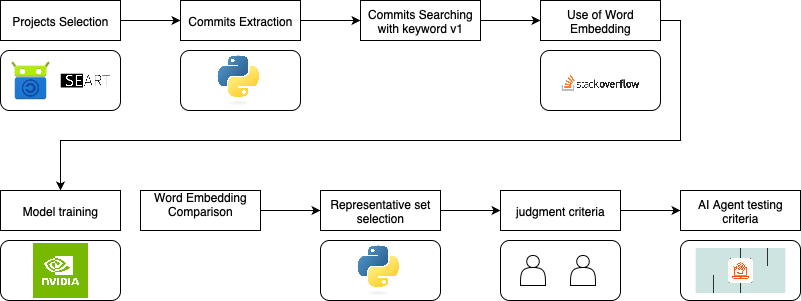
\includegraphics[scale=0.5]{/Users/juancamiloacosta/Documents/uniandes/tesis 2/thesis template repo/master-thesis-document/thesis-template/figures/workflow-3-ASE.png}
   			 \caption{seART platform for GitHub repositories searching \cite{} }
   			 \label{fig:ast}
\end{figure}

\subsection{Commits Extraction}
The first process is the extraction of a set of commits to evaluate and identify AER issues. We implemented the same methodology for the static code analysis solution approach. We used the same sampled Android projects and used their large set of commits to explore new keywords based on different Word Embedding models.

\subsubsection{Applications selections}
We used two platforms to build the Android application set: GHS from SEART and FDroid \cite{seart,fdroid}. GHS is a repository mining platform of GitHub repositories developed by SEART. We implemented different filters to get some Android applications to the AER issues evaluation. The filters were based on the number of commits (between 1000 and more than 20000 commits), the main programming language as Kotlin, and the date of the last commit. These filters were implemented to gather sufficient information for analyzing the presented AER issues in code fragments written in the Kotlin programming language.
The second used platform was FDroid. FDroid is an open-source marketplace with Android applications. FDroid provides some important information about every Android project, like GitHub repository URL and the software license. We randomly extracted s subset of Android applications to add to the previous set of applications extracted from GHS. Summarizing, we extracted a set of 50 Android applications to analyze their commits and perform NLP processing to identify new potential keywords related to the AER phenomenon.

There are some practices and techniques for repository mining. Repository mining allows the finding of relevant information from any source code repository in any versioning platform like GitHub, GitLab, BitBucket, etc. Some tools and libraries have been developed for this purpose. The selected library for this is the PyDriller library \cite{pydriller}.  PyDriller can extract relevant information from each commit, like project name, commit hash, modified source code, etc. We define a common structure to build the commits dataset. This is shown in Table xxxx.  With the defined structure, we implement a Python program to extract from the GitHub repositories of each Android project. The execution of the program generated a dataset of more than 470000 GitHub commits. The commits were filtered if each one contained or not one of the keywords defined in the previous steps.

\subsection{Use of Word Embedding Models}
With the generated dataset of commits. It is possible to explore some alternatives based on NLP techniques. One of them is the use of Word Embedding models. These models help to get a numerical representation of the words in specific or dynamic contexts. Numerical representation of words helps in computer processing and metrics building. With the two different types of Word Embedding models, we explored the definition of the most similar keywords from the previous set. In the workflow, we defined the use of two approaches to identify new AER keywords: using static and dynamic Word Embedding models.

\subsubsection{Static Word Embedding Models}
Static Word Embedding models are limited by their training context. We considered the well-known Word Embedding models for text processing, and one Word Embedding trained with a large set of Stack Overflow posts, named the SO model. We implemented NLP techniques like lemmatization and stop word removal, and used three static Word Embedding models: Glove, Word2Vec, and the SO model. We calculate the cosine similarity average to get the top 10 most similar words of each Word Embedding model. We realized the comparison between each Word Embedding model according to the average cosine similarity. Another approach used was to calculate the top 10 most similar words for each keyword of the previous set. However, a large set of words was selected, and some of them were not related to the technological context and the main objective of the methodology. We defined an embedding dimension of 200, which is a standard model for the three analyzed Word Embedding models. Furthermore, we considered a sufficient dimension to represent the words in a specific context.


\subsubsection{Dynamic Word Embedding Models}
Due to the limited resources of static Word Embedding models, it is necessary to explore additional alternatives to get an improvement with respect to the context of those models. For this, we considered the use of AI models that are trained for code classification and generation. Models like CodeBERT and T5 are small and effective models to classify and generate code based on different training strategies, like code masking, to predict the right keyword in any code fragment \cite{codebert,t5}.  
CodeBERT is a model that is considered an autoencoder. It can receive different inputs and can generate different outputs for different learning tasks. CodeBERT has distilled models like CodeReviewer, CodeGraph, etc. Distilled models are able to resolve individual learning tasks. In the case of CodeReviewer, its main learning task is to classify code as code that needs review or not. Another learning task in CodeReviewer is the review generation of code in natural language and code refinement. Based on the review code task, we can extend and implement fine-tuning of the model according to the set of commits of the Android projects, and evaluate the model for AER issues detection according to the commit messages and the code changes of every commit \cite{codereviewer, codegraph}. 



\subsection{Testing the models}
We analyzed the results obtained from the use of static and dynamic Word Embedding models. We will present the results of the extracted words of every model and the performance metrics in the case of the CodeReviewer fine-tuning process. We will make a comparison between the use of the two types of Word Embedding models for identifying AER issues. Furthermore, we will define the advantages and the disadvantages of the use of AI models and NLP techniques for AER issues identification. We will define the possible extension of the use of this methodology for issues identification for other quality attributes in software engineering 

\section{Methodology Implementation}

\subsection{Commits Extraction}
We used the commit extraction process outlined in the methodology, based on static code analysis. We used the selected Android applications extracted from the mentioned platforms \cite{seart,fdroid}. After that, we used the PyDriller library to extract the commits from the GitHub repository of each Android project \cite{pydriller}.  As an additional step, we implemented tagging based on the commit message of each row. If the commit contains one of the initial set of selected keywords, the commit will be tagged as 1. Otherwise, the commit will be tagged as 0. This is for an initial tagging for the fine-tuning process with the CodeReviewer model.


\subsection{Word Embedding Models Results}
We implemented each type of word embedding model. For static word embedding models, we extracted the top 10 words and the most similar words of each model to make a comparison of the effectiveness of each model. In the case of the dynamic word embedding model, we extracted the effectiveness with a sample extracted from the large set of commits of the Android projects. Furthermore, we extracted the top 10 most similar words, based on the cosine similarity metric, averaged with respect to the initial set of keywords. 
Those results will be tested with an AI agent implementation with the GPT4-o LLM model \cite{gpt4reference}. The AI agent tagged a sample of evaluated GitHub commits used for the CodeReviewer fine-tuning process for measuring the performance obtained with the CodeReviewer model in AER issues identification


\subsubsection{Static Word Embedding Models}
We presented the most similar words based on the cosine similarity metric, averaged with the initial set of keywords. Additionally, we presented the most similar keywords found by every word embedding model. The top 10 most similar words were shown in the methodology based on static code analysis.

\begin{table}
[htbp]
    \setlength{\tabcolsep}{1.5pt}
    \resizebox{\textwidth}{!}{\begin{tabular}{|l*{56}{c|}}
        \toprule
        \textbf{Word} & \rotatebox{90}{\textbf{general}} & \rotatebox{90}{\textbf{respect}} & \rotatebox{90}{\textbf{design}} & \rotatebox{90}{\textbf{notion}} & \rotatebox{90}{\textbf{common}} & \rotatebox{90}{\textbf{complex}} & \rotatebox{90}{\textbf{formal}} & \rotatebox{90}{\textbf{depend}} & \rotatebox{90}{\textbf{adopt}} & \rotatebox{90}{\textbf{differ}} & \rotatebox{90}{\textbf{hing}} & \rotatebox{90}{\textbf{to-do}} & \rotatebox{90}{\textbf{borderless}} & \rotatebox{90}{\textbf{christian}} & \rotatebox{90}{\textbf{rend}} & \rotatebox{90}{\textbf{list}} & \rotatebox{90}{\textbf{misc}} & \rotatebox{90}{\textbf{non-act}} & \rotatebox{90}{\textbf{contributor}} & \rotatebox{90}{\textbf{wiki}} & \rotatebox{90}{\textbf{conform}} & \rotatebox{90}{\textbf{disregard}} & \rotatebox{90}{\textbf{mismatch}} & \rotatebox{90}{\textbf{implement}} & \rotatebox{90}{\textbf{distinct}} & \rotatebox{90}{\textbf{contradict}} & \rotatebox{90}{\textbf{non-standard}} & \rotatebox{90}{\textbf{rigid}} \\
        \midrule
        \textbf{SO model} & 0.31 & 0.3 & 0.29 & 0.28 & 0.266 & 0.265 & 0.264 & 0.262 & 0.262 & 0.26 & 0 & 0 & 0 & 0 & 0 & 0 & 0 & 0 & 0 & 0 & 0 & 0 & 0 & 0 & 0 & 0 & 0 & 0 \\
        \textbf{Glove model} & 0 & 0 & 0 & 0 & 0 & 0 & 0 & 0 & 0 & 0 & 0.1019 & 0.1017 & 0.1 & 0.09 & 0.086 & 0.085 & 0.083 & 0.081 & 0.0809 & 0.802 & 0 & 0 & 0 & 0 & 0 & 0 & 0 & 0 \\
        \textbf{Word2Vec model} & 0 & 0 & 0.2379 & 0 & 0 & 0 & 0 & 0 & 0 & 0.2269 & 0 & 0 & 0 & 0 & 0 & 0 & 0 & 0 & 0 & 0 & 0.2382 & 0.231 & 0.23 & 0.2298 & 0.22292 & 0.2291 & 0.2280 & 0.2263\\
        \bottomrule
    \end{tabular}}
    \label{tab:my_label}
    \caption{Cosine similarity between Static Word Embedding models}
\end{table}

The model with the most extracted words related to the technological context is the SO model. The other models, like Word2Vec and the Glove model, show more words in "natural language", due to the context used for their training. In the case of static word embedding models, it is very important to define the training context and the dimension. The SO model can be considered an important model to explore more issues and warnings in commit messages.


\subsubsection{Dynamic Word Embedding Models}
For the implementation of dynamic word embedding models, we used an Nvidia GPU with 16GB of memory. We used CUDA for GPU processing for machine learning tasks and AI models management \cite{cuda}. We loaded the CodeReviewer model with the PyTorch library \cite{pytorch} and selected a sample of the commits set of the Android projects. The commits selected were around 148K commits, with 50\% of the commits tagged as  0 (no containing any keyword of the initial set of keywords), and the other ones were tagged as 1 (containing one or more keywords of the initial set of keywords). We divided the data into training data, validation data, and test data. 70\% of commits were used as training data, 15\% used as validation data, and the other 15\% used as testing data. We implemented the fine-tuning model of CodeReviewer with 3 epochs. We extracted the model performance with respect to the testing data and the tagging criteria (considered as a first approach to select any commit as an AER issue).


\begin{table}[h]
    \centering
    \begin{tabular}{|c|c|c|c|}
        \hline
        Class & Precision & Recall & F1-Score \\
        \hline
        0 & 93\% & 94\% & 93\% \\
        \hline
        1 & 94\% & 93\% & 93\% \\
        \hline
    \end{tabular}
     \caption{metrics of Codereviewer with respect to test data in AER issues classification}
    \label{tab:my_label}
\end{table}

When the fine-tuning process finished. We extracted the tokenizer and the dynamic word embedding model that contains the CodeReviewer model. In the same case as the evaluation of static word embedding models, we selected the most similar words according to the cosine similarity metric averaged with the initial set of keywords.

\begin{table}[h]
    \centering
    \begin{tabular}{|c|c|}
    \hline
       Word  & Cosine Similarity \\
    \hline
        layout & 0.4696 \\
        \hline
        concept & 0.4535 \\
        \hline
        package & 0.4523 \\
        \hline
        controller & 0.4483 \\
        \hline
        settings & 0.4440 \\
        \hline
        generic & 0.4414 \\
        \hline
        interface & 0.4414 \\
        \hline
        element & 0.4393 \\
        \hline
        application & 0.4281 \\
        \hline
        purpose & 0.4280 \\
    \hline
    \end{tabular}
    \caption{Keywords found in the word embedding model of the trained CodeReviewer model}
    \label{tab:my_label}
\end{table}

With these results, we can define a performance metric based on the evaluation of an AI Agent. We implemented with the OpenAI library an agent that used the GPT4-o LLM. We implemented some calls to evaluate a sample of commits evaluated in the CodeReviewer model with a customized prompt that gave the AI agent a specific context.

\begin{lstlisting}[caption={Defined prompt for AI evaluation}, label={pr:prompt}, basicstyle=\ttfamily\small, breaklines=true]
You are an expert in software architecture for Android applications written in the Kotlin programming language.

You will receive a code fragment extracted from a GitHub commit in an Android app repository. This code fragment contains only the lines that were changed during the commit:

- Lines starting with `+` represent **added code**.
- Lines starting with `-` represent **removed code**.

Your task is to analyze **only the lines that were added or removed**, and determine whether the changes introduce or contribute to **architectural erosion**.

Architectural erosion refers to the progressive degradation of a system's design and structure due to poor development practices. It can be caused by:

- Violations of SOLID principles
- High coupling between modules or components
- Dispersion of business logic
- Repetitive or duplicated changes across multiple architectural layers
- Leaking logic between layers (e.g., UI handling persistence directly)
- Adding code without tests or separation of concerns
- Implementation of blocking functions in asynchronous contexts
- Poor or missing exception handling
- Improper exception handling within ViewModel classes

Return only a number:
- 1 if the **added or removed code** could introduce architectural erosion
- 0 if not

Code to analyze:
```kotlin
code
```
\end{lstlisting}
	
 We randomly selected 200 commits for evaluation, constrained by cost limits that restricted the data volume. Commits were chosen based on their length in lines of code. For each commit, we compared the AI-generated labels with those produced by CodeReviewer. The AI agent achieved an accuracy of 55\%, which represents a promising initial result for this type of learning task. Further improvements could be achieved by increasing the dataset size and refining both the CodeReviewer annotations and the use of smaller, specialized AI models.


